%This was done for SDP lab assignment 3
\documentclass[titlepage]{article}
\usepackage[T1]{fontenc}
\usepackage{pgf-umlcd}

%to change default behavior
\renewcommand{\unidirectionalAssociation}[4]
{
  \draw[umlcd style, ->] (#1) -- (#4)
  node[near end, auto]{#2}
  node[near end, auto,swap]{#3};
}

\renewcommand{\aggregation}[4]
{
  \draw[umlcd style, -open diamond] (#1) -- (#4)
  node[near end, auto]{#2}
  node[near end, auto,swap]{#3};
}

\usepackage[a4paper,textwidth=8in]{geometry}
\begin{document}
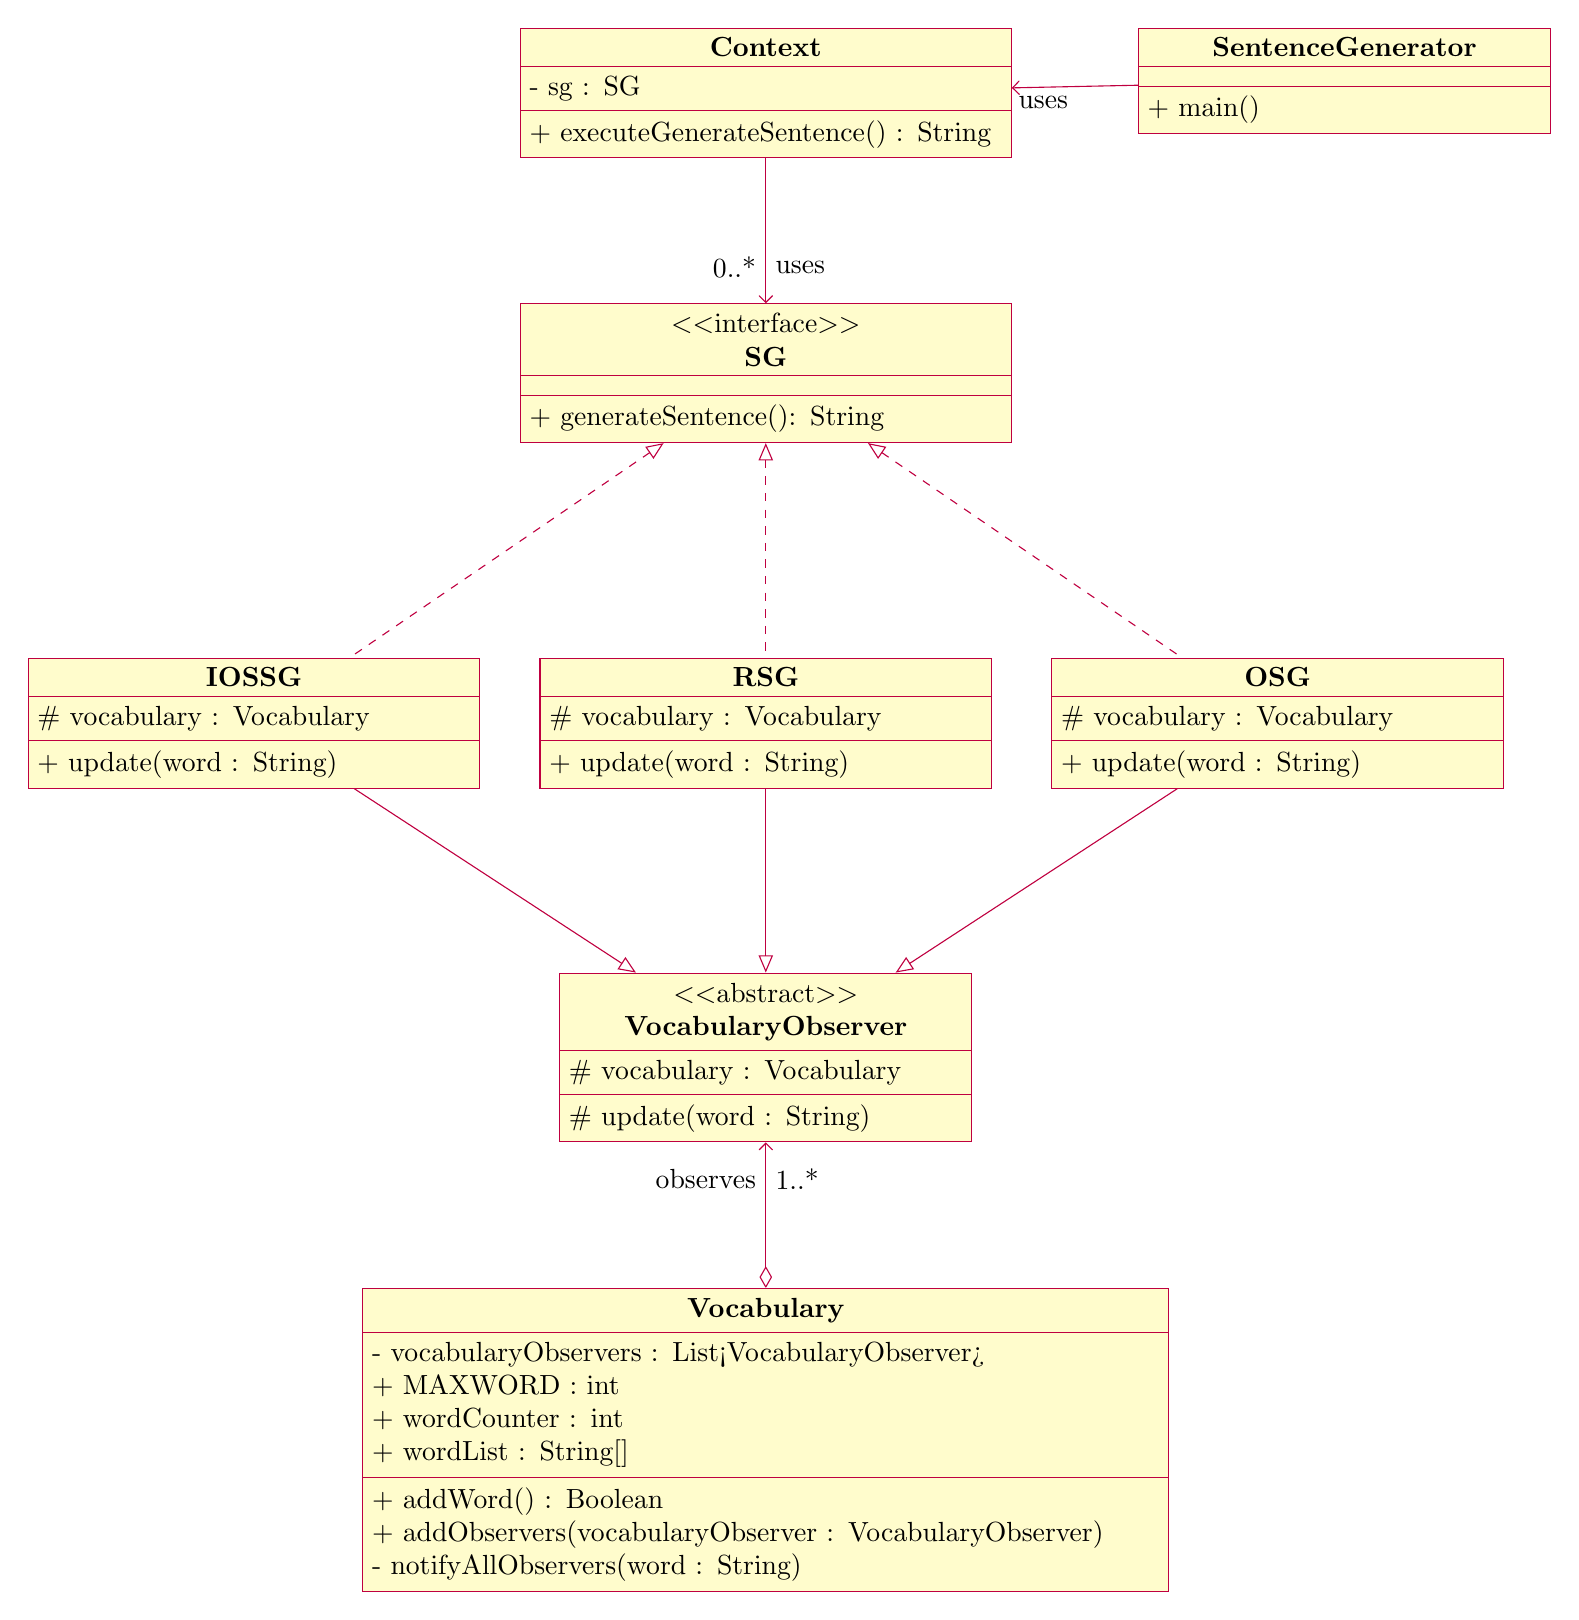
\begin{tikzpicture}

  \begin{interface}[text width = 6cm]{SG}{1.5,2.5}
    \operation{+ generateSentence(): String}
  \end{interface}


  \begin{abstractclass}{VocabularyObserver}{1.5, -6}
    \attribute{\# vocabulary : Vocabulary}
    \operation{\# update(word : String)}
  \end{abstractclass}
  
  \begin{class}[text width = 10 cm]{Vocabulary}{1.5,-10}
    \attribute{- vocabularyObservers : List<VocabularyObserver>}
    \attribute{+ MAXWORD : int}
    \attribute{+ wordCounter : int}
    \attribute{+ wordList : String[]}
    \operation{+ addWord() : Boolean}
    \operation{+ addObservers(vocabularyObserver : VocabularyObserver)}
    \operation{- notifyAllObservers(word : String)}
  \end{class}

  \begin{class}[text width = 5.5cm]{RSG}{1.5,-2}
    \implement{SG}
    \inherit{VocabularyObserver}
    \attribute{\# vocabulary : Vocabulary}
    \operation{+ update(word : String)}
  \end{class}

  \begin{class}[text width = 5.5cm]{IOSSG}{-5,-2}
    \implement{SG}
    \inherit{VocabularyObserver}
    \attribute{\# vocabulary : Vocabulary}
    \operation{+ update(word : String)}
  \end{class}

  \begin{class}[text width = 5.5cm]{OSG}{8,-2}
    \implement{SG}
    \inherit{VocabularyObserver}
    \attribute{\# vocabulary : Vocabulary}
    \operation{+ update(word : String)}
  \end{class}

  \begin{class}[text width = 6 cm]{Context}{1.5,6}
    \attribute{- sg : SG}
    \operation{+ executeGenerateSentence() : String}
  \end{class}

  \begin{class}{SentenceGenerator}{8.85,6}
    \operation{+ main()}
  \end{class}
\unidirectionalAssociation{Context}{uses}{0..*}{SG}
\unidirectionalAssociation{SentenceGenerator}{uses}{}{Context}
  \aggregation{Vocabulary}{observes}{1..*}{VocabularyObserver}
\end{tikzpicture}
\end{document}
